\newcommand{\CODELOC}{c/ch7/}

\chapter{Poisson PDE by an unstructured FEM method}
\label{chap:unstructured}

The cliched Poisson problem can be exploited some more.  It gives us the opportunity to use \PETSc for important tasks we have not yet seen, including reading an unstructured mesh into \PETSc \pVecs, symmetric implementation of boundary conditions, and explicit preallocation of a \pMat in parallel.

\section{Example: The Poisson problem}

Let $\Omega \subset \RR^d$ be a bounded (open) region.  Suppose its boundary $\partial\Omega$ is well-behaved, for instance that it is Lipschitz-continuous \citep[section 1.2]{Ciarlet} or even polygonal.  Suppose $\partial\Omega$ is decomposed into (measurable) disjoint subsets $\partial_D \Omega$ and $\partial_N \Omega$ whose union is the entire boundary $\partial \Omega$.  The \emph{Poisson problem}, in strong form and including nonhomogeneous Dirichlet and Neumann boundary conditions, is\marginnote{%
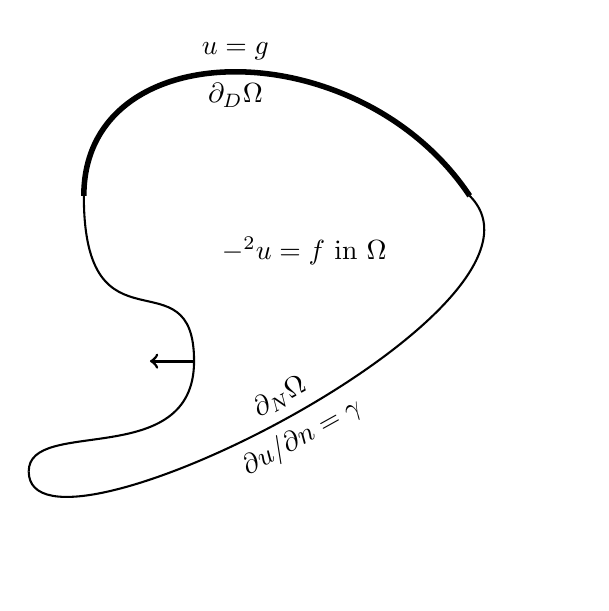
\begin{tikzpicture}[scale=0.7]
%\draw[gray,very thin] (-2,-6) grid (8,3);
\draw[line width=2pt] (0,0) .. controls (0,3) and (5,3) .. node[sloped,above] {$u=g$} node[sloped,below] {$\partial_D\Omega$} (7,0);
\draw[line width=0.75pt] (7,0) .. controls (9,-2) and (-1,-7) .. node[sloped,above] {$\partial_N\Omega$} node[sloped,below] {$\partial u/\partial n = \gamma$} (-1,-5);
\draw[line width=0.75pt] (-1,-5) .. controls (-1,-4) and (2,-5) .. (2,-3);
\draw[line width=0.75pt] (2,-3) .. controls (2,-1) and (0,-3) .. (0,0);
\draw[->,line width=1.0pt] (2,-3) -- (1.2,-3) node[below] {$\bn$}; % normal vector
\draw (4,-1) node {$- \grad^2 u = f$ in $\Omega$};
\end{tikzpicture}}
\begin{align}
- \grad^2 u &= f \quad \text{ on } \Omega, \label{poissonstrong} \\
u &= g \quad \text{ on } \partial_D \Omega, \notag \\
\frac{\partial u}{\partial n} &= \gamma \quad \text{ on } \partial_N \Omega \notag
\end{align}
where $\bn$ is the outward unit normal on $\partial \Omega$ and $\partial u/\partial n = \bn \cdot \grad u$.  The data of problem \eqref{poissonstrong}, besides the region $\Omega$ and its boundary, includes a \emph{source term} $f\in L^2(\Omega)$, \emph{Dirichlet data} $g\in L^2(\partial_N \Omega)$, and \emph{Neumann data} $\gamma\in L^2(\partial_N \Omega)$.

As \eqref{poissonstrong} is stated there may be no solution where ``$\grad^2 u$'' makes sense as a continuous function, even for polygonal regions, continuous boundary values, and continuous source functions.  In particular, there may be no $u\in C^2(\Omega)$ which is continuous up to the boundary (i.e.~$u\in C(\bar\Omega)$) and so that $\grad^2 u = f$.  There is, however, a solution if we change to a \emph{weak formulation}.\sidenote{A proof of this well-posedness claim is in \citet{Ciarlet} and in \citet{Evans}.  These are technicalities for us, however, as our goal is computational performance in cases where the Poisson problem is mathematically well-behaved and easily approximated.}  Furthermore, if $\partial_D \Omega$ has positive size, in an appropriate sense \citep[Theorem 1.2.1]{Ciarlet}, then the solution of the weak formulation is unique.  We will state the weak formulation after glossing the definitions of the needed function spaces.

Recalling $L^2(\Omega)$ is the space of all square-integrable real functions on $\Omega$, define
    $$H^1(\Omega) = \{u\in L^2(\Omega) \big| \grad u \text{ exists a.e.~and } \grad u \in L^2(\Omega)\},$$
which is a Sobolev space \citep{Evans}.  This space has two subsets we use, namely functions with value $g$ on $\partial_D \Omega$ and those with value $0$ on $\partial_D \Omega$, respectively, which we denote $H_g^1(\Omega)$ and $H_0^1(\Omega)$.  Note that $H_0^1(\Omega)$ is a linear subspace of $H^1(\Omega)$.  While $H_g^1(\Omega)$ is generally not a subspace (e.g.~because the zero function is not in it), it is an affine subspace, and we refer to both $H_g^1(\Omega)$ and $H_0^1(\Omega)$ as ``subspaces''.

To get to the weak formulation of the Poisson problem we suppose we already have a classical solution $u$ of \eqref{poissonstrong}.  Then we choose any $v\in H_0^1(\Omega)$, multiply the first equation in \eqref{poissonstrong} by $v$, and integrate by parts:
\begin{equation*}
\int_\Omega \grad u \cdot \grad v - \int_{\partial\Omega} \frac{\partial u}{\partial n} v = \int_\Omega f v.
\end{equation*}
Next\marginnote{%
{\color{red}Main ideas} of strong and weak formulations:\begin{itemize}
\item If $u \in H_g^1(\Omega)$ solves the strong form \eqref{poissonstrong} then it solves \eqref{poissonweak} also.
\item If $u \in H_g^1(\Omega)$ solves the weak form \eqref{poissonweak} then we accept it, by definition, as a solution of the Poisson problem.\end{itemize}} 
we use the other data, namely that $v=0$ on $\partial_D\Omega$ and that there is Neumann data $\gamma$ on $\partial_N\Omega$:
\begin{equation}
\int_\Omega \grad u \cdot \grad v = \int_\Omega f v + \int_{\partial_N\Omega} \gamma v\quad \text{ for any } v\in H_0^1(\Omega). \label{poissonweak}
\end{equation}

Equation \eqref{poissonweak} is the weak formulation of the Poisson problem.  Any $u \in H_g^1(\Omega)$ satisfying \eqref{poissonweak} is called a \emph{weak solution}.  A key observation is that $u$ itself incorporates the Dirichlet boundary condition, because it lives in $H_g^1(\Omega)$, while both the Neumann boundary data $\gamma$ and the source function $f$ appear in equation \eqref{poissonweak}.


\section{A finite element method (FEM) for the Poisson problem in the plane}

An FEM for the Poisson problem comes from requiring the weak formulation \eqref{poissonweak} to be true for $u$ in a much smaller, indeed finite-dimensional, subspace of $H_g^1(\Omega)$, and for test functions $v$ ranging over a finite-dimensional subspace of $H_0^1(\Omega)$.  In the ``Galerkin'' method here, these subspaces will be essentially the same.  We will build these subspaces, in the current example, using an unstructured triangulation on $\Omega\subset \RR^2$; from now on in this Chapter we restrict to $d=2$ dimensions.

Furthermore, to make our finite-dimensional spaces true subspaces of $H^1(\Omega)$---to make our FEM \emph{conforming}---we require that $\Omega$ be polygonal, with $\partial\Omega$ a closed polygon.  Segments of $\partial\Omega$ must have positive length, and be either entirely in $\partial_D\Omega$ or entirely in $\partial_N\Omega$.  We also assume $\partial_D\Omega$ is a closed set so that, at vertices of $\partial \Omega$ where the Dirichlet boundary and Neumann boundary meet, the vertex is Dirichlet.

By definition, a \emph{triangulation} is a finite set of non-overlapping, non-empty open triangles $\triangle_k\subset \RR^2$ which tile $\Omega$:
\begin{equation*}
\Th = \left\{\triangle_k \quad\Big|\quad \cup_k \overline{\triangle}_k = \overline{\Omega} \quad \text{ and} \quad \Omega_k \cap \Omega_l = \emptyset \text{ if } k\ne l\right\}.
\end{equation*}
We index the $K$ triangles in $\Th$ by $k=0,\dots,K-1$.  The $N$ vertices (nodes) in $\Th$ are indexed by $j=0,1,\dots,N-1$, with locations
\begin{equation*}
\bx_j = (x_j,y_j).
\end{equation*}
An example triangulation is shown in Figure \ref{fig:number-elements}.

\begin{marginfigure}
\input{samplepoly.1.tikz}
\caption{A triangulation $\Th$ with $K=22$ triangles (elements) numbered $k=0,1,\dots,K-1$ ({\color{red} red}) and $N=16$ nodes numbered $j=0,1,\dots,N-1$  ({\color{blue} blue}).  Nodes $\bx_0$, $\bx_1$, $\bx_2$, $\bx_3$ are in the Dirichlet boundary $\partial_D\Omega$.}
\label{fig:number-elements}
\end{marginfigure}

For now the reader can regard the subscript ``$h$'' in ``$\Th$'' as merely-traditional notation.  It denotes the typical or maximum size $h$ (e.g.~diameter) of the triangles, and it serves as a reminder that we want to approximate the solution in the limit $h\to 0$.  Also note that, in contrast to \citet{Elmanetal2005}, which we generally follow, and other references on the FEM or its implementation in languages like \Matlab, our indexing is zero-based.  This is so because we implement in C and we want to avoid any confusion when comparing text and codes.  Breaking long mathematical traditions, rows and columns of vectors and matrices will also have numbering starting with zero in this book.

We informally call the triangles \emph{elements}, though there is more to the definition of ``element.''  We are going to approximate the Poisson problem with $\Pone$ finite elements, which means that our finite-dimensional subspace contains only piecewise-linear functions which are linear on each triangle $\triangle_k$.

For each node $j$ there is a $\Pone$ basis function, or ``hat'' function, $\phi_j(x,y)$ which is linear on each triangle, continuous on all of $\overline{\Omega}$, and equal to one on only one node $j$:\marginnote{%
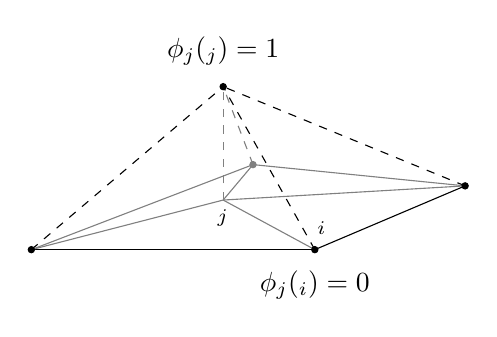
\begin{tikzpicture}[scale=0.9, z={(.707,.3)}]
    % (2,2,1) is top
    \draw[style=dashed] (0,0,0) -- (2,2,1); % to top from left
    \draw[style=dashed] (4,0,0) -- (2,2,1); %   ...  from front
    \draw[style=dashed] (4,0,3) -- (2,2,1); %   ...  from right
    \draw[color=gray, style=dashed] (0.3,0,4) -- (2,2,1); % from back
    \draw[color=gray, style=dashed] (2,0.4,1) -- (2,2,1); % from middle
    % draw base
    \draw (0,0,0) -- (4,0,0);
    \draw (4,0,0) -- (4,0,3);
    \draw[color=gray] (0,0,0) -- (0.3,0,4);
    \draw[color=gray] (0.3,0,4) -- (4,0,3);
    \draw[color=gray] (0,0,0) -- (2,0.4,1);
    \draw[color=gray] (2,0.4,1) -- (4,0,3);
    \draw[color=gray] (4,0,0) -- (2,0.4,1);
    \draw[color=gray] (2,0.4,1) -- (0.3,0,4);
    % draw \phi_j at nodes
    \filldraw (2,2,1) circle (1.25pt);
    \draw (2,2.5,1) node {$\phi_j(\bx_j)=1$};
    \draw (2,0.15,1) node {$\bx_j$};
    \filldraw (0,0,0) circle (1.25pt);
    \filldraw (4,0,0) circle (1.25pt);
    \draw (4,-0.5,0) node {$\phi_j(\bx_i)=0$};
    \draw (4.1,0.3,0) node {$\bx_i$};
    \filldraw (4,0,3) circle (1.25pt);
    \filldraw[color=gray] (0.3,0,4) circle (1.25pt);
\end{tikzpicture}
}%
\begin{equation*}
\phi_j(\bx_i) = \delta_{ij}.
\end{equation*}
The functions $\phi_j$ are in $H^1(\Omega)$, with piecewise-constant partial derivatives $\partial\phi_j/\partial x$ and $\partial\phi_j/\partial y$.  Also, the set $\{\phi_j\}_{j=0,\dots,N-1}$ is linearly-independent.  On each triangle, $\phi_j$ has three degrees of freedom, because on $\triangle_k$ there exist coefficients $A_k,B_k,C_k\in\RR$ so that
\begin{equation*}
\phi_j(\bx) = A_k + B_k x + C_k y \quad \text{ on } \triangle_k,
\end{equation*}
where $\bx = (x,y)$.

We can immediately use these basis functions to approximate the Dirichlet data $g$ and extend it to the region $\Omega$.  We will assume from now on that the Dirichlet boundary $\partial_D\Omega$ is closed, and index the $L$ nodes which are in the Dirichlet boundary by $\bx_{j_l} \in \partial_D\Omega$ for $l=0,\dots,L-1$.  (Figure \ref{fig:number-elements} shows an example with $L=4$ and $j_l=l$ for $l=0,1,2,3$, but any subset of boundary points can be Dirichlet as long as the index values $j_l$ are well-defined.)  Now we can define an extended interpolant $\hat g$ of $g$ as the function which has the correct value on the Dirichlet boundary nodes and which extends to all of $\Omega$ in a continuous and piecewise-linear way:
\begin{equation}
\hat g(\bx) = \sum_{l=0,\dots,L} g(\bx_{j_l}) \phi_{j_l}(\bx). \label{hatgdefine}
\end{equation}

By using $\hat g$ and the basis functions $\phi_j$, we can now describe three finite-dimensional subspaces of $H^1(\Omega)$:\sidenote{Traditionally, basis functions for $S_g^h$ are called the \emph{trial} functions, and basis functions for $S_0^h$ are called \emph{test} functions.  We will generally just use the labels ``$S_g^h$'' and ``$S_0^h$.''}
\begin{align*}
S^h &= \Span\{\phi_j \,\big|\, \text{ all } j\,\}, \\
S_0^h &= \Span\{\phi_j \,\big|\, \bx_j \notin \partial_D \Omega\} \subset S^h, \\
S_g^h &= S_0^h + \hat g \subset S^h.
\end{align*}
Then $\dim(S^h)=N$ while $\dim(S_0^h)=\dim(S_g^h)=N-L$, with $S_g^h$ only an affine subspace of $S^h$.

Our FEM requires that the weak formulation  \eqref{poissonweak} be true of $u_h\in S_g^h$ for all $v\in S_0^h$.  Thus we first write $u_h$ in the basis for $S_g^h$ using $N-L$ unknown coefficients $u_j$:
\begin{equation}
u_h(\bx) = \hat g(\bx) + \sum_{\bx_j \notin \partial_D \Omega} u_j\, \phi_j(\bx). \label{uhexpand}
\end{equation}
Then we require that the weak formulation hold for all $\phi_i$ in the basis of $S_0^h$.  That is, using definition \eqref{hatgdefine} and expansion \eqref{uhexpand}, we require
\begin{align}
\sum_{\bx_j \notin \partial_D \Omega} u_j \int_\Omega \grad \phi_j \cdot \grad \phi_i &= \int_\Omega f \phi_i + \int_{\partial_N\Omega} \gamma \phi_i \label{poissonfem} \\
&\qquad - \sum_{l=0,\dots,L} g(\bx_{j_l})  \int_\Omega \grad \phi_{j_l} \cdot \grad \phi_i \notag
\end{align}
for all $i$ such that $\bx_i \notin \partial_D \Omega$.  The coefficients $u_j$, for all $j$ such that $\bx_j \notin \partial_D \Omega$, are the unknowns in this equation.

Note that the support (i.e.~nonzero set) of $\phi_j$ includes only the node $\bx_j$ and all triangles (elements) $\triangle_k$ for which $\bx_j$ is a node of $\triangle_k$.  Thus the integral ``$\int_\Omega \grad \phi_j \cdot \grad \phi_i$'' in \eqref{poissonfem} is usually zero.  Specifically, it is zero if $\bx_i$ and $\bx_j$ are not both nodes of at least one triangle in the triangulation.


\section{Triangular meshes from \Triangle}

\PETSc itself does not include any tools for triangulating regions of the plane, sowe use the widely-available and easy-to-use \Triangle\sidenote{See \href{http://www.cs.cmu.edu/~quake/triangle.html}{www.cs.cmu.edu/$\sim$quake/ triangle.html} for documentation and source code. \Triangle may be available as a package in your operating system.} software \citep{Shewchuk1996} for this task.  \Triangle is both limited to planar regions and only capable of writing ASCII files.  Thus it is not a choice for performance, but of convenience.

\Triangle uses a simply-formatted ASCII file (extension \texttt{.poly}) as input to describe a polygonal region $\Omega$, and to indicate Dirichlet and Neumann portions of the boundary $\partial \Omega$.  For example, consider the input file \texttt{bump.poly} shown in Figure \ref{code:bumppoly}.  This example polygon, a rectangle with a triangular bump in the base, is shown in Figure \ref{fig:bump-poly}.  It will reappear several times in this book as we solve more interesting PDEs on it.  The two apparently-unnecessary vertices introduced along the bottom help identify the Neumann part of the boundary, but note that \texttt{bump.poly} includes a Dirichlet/Neumann flag along each boundary segment.

\inputfromline{../\CODELOC/bump.poly}{bump.poly}{A description of the boundary polygon in Figure \ref{fig:triangulation}, suitable for reading by \Triangle.}{16}{code:bumppoly}

The triangulation shown in Figure \ref{fig:triangulation} came from a single command which asks \Triangle to take \texttt{bump.poly} and generate a triangulation which has a polygon output file (option \texttt{-p}), relatively-uniform triangles (option \texttt{-q} for ``quality-checked'' \citep{Shewchuk1996}), and triangles with maximum area of $1.0$ (option \texttt{-a1.0}):
\begin{marginfigure}
\input{bump.poly.tikz}
\caption{The polygon described by \texttt{bump.poly} in Figure \ref{code:bumppoly}.  The bold part is the closed Dirichlet boundary.  The lower boundary is Neumann, and has ``extra'' nodes to identify it as such.}
\label{fig:bump-poly}
\end{marginfigure}
\begin{cline}
$ triangle -pqa1.0 bump
\end{cline}
%$
This command generates three ASCII files, \texttt{bump.1.poly}, \texttt{bump.1.node}, and  \texttt{bump.1.ele}.  These files define the new (i.e.~refined relative to \texttt{bump.poly}) polygonal boundary, the nodes locations, and the elements in the triangulation, respectively.  For example, \texttt{bump.1.node} has the numbering and node locations shown in blue in Figure \ref{fig:triangulation}.

\Triangle includes a minimal visualization tool which shows the triangulation graphically.  The command
\begin{cline}
$ showme bump
\end{cline}
%$
displays the boundary polygon (from \texttt{bump.poly} or \texttt{bump.1.poly}) and the triangulation itself (\texttt{bump.1.node} and \texttt{bump.1.ele}).

\begin{figure}
\bigskip
% created by script tri2tikz.py command line:
%   ./tri2tikz.py --labelnodes --scale 2.0 --labeloffset 0.25 bump.1 bump.1.tikz
%
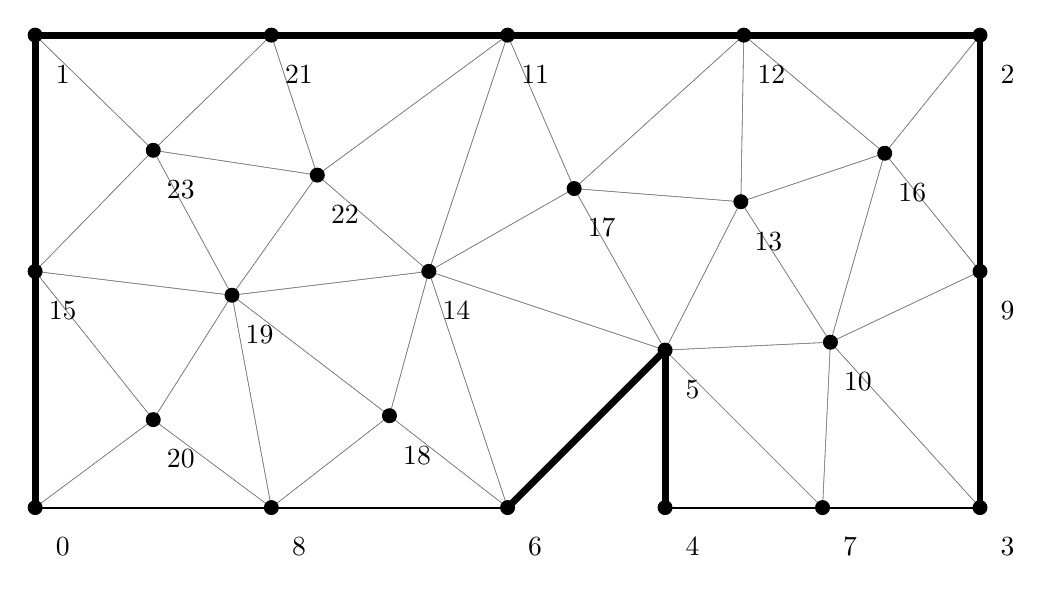
\begin{tikzpicture}[scale=2.000000]
  \draw[gray,very thin] (-1.500000,0.000000) -- (-2.250000,0.558372);
  \draw[gray,very thin] (-2.250000,0.558372) -- (-3.000000,0.000000);
  \draw[gray,very thin] (-3.000000,0.000000) -- (-1.500000,0.000000);
  \draw[gray,very thin] (-1.500000,0.000000) -- (0.000000,0.000000);
  \draw[gray,very thin] (0.000000,0.000000) -- (-0.750000,0.583333);
  \draw[gray,very thin] (-0.750000,0.583333) -- (-1.500000,0.000000);
  \draw[gray,very thin] (1.481325,1.942169) -- (0.422665,2.025778);
  \draw[gray,very thin] (0.422665,2.025778) -- (1.000000,1.000000);
  \draw[gray,very thin] (1.000000,1.000000) -- (1.481325,1.942169);
  \draw[gray,very thin] (-0.500000,1.500000) -- (0.000000,0.000000);
  \draw[gray,very thin] (0.000000,0.000000) -- (1.000000,1.000000);
  \draw[gray,very thin] (1.000000,1.000000) -- (-0.500000,1.500000);
  \draw[gray,very thin] (0.000000,3.000000) -- (-1.500000,3.000000);
  \draw[gray,very thin] (-1.500000,3.000000) -- (-1.208263,2.111158);
  \draw[gray,very thin] (-1.208263,2.111158) -- (0.000000,3.000000);
  \draw[gray,very thin] (2.000000,0.000000) -- (2.050000,1.050000);
  \draw[gray,very thin] (2.050000,1.050000) -- (1.000000,1.000000);
  \draw[gray,very thin] (1.000000,1.000000) -- (2.000000,0.000000);
  \draw[gray,very thin] (1.000000,0.000000) -- (2.000000,0.000000);
  \draw[gray,very thin] (2.000000,0.000000) -- (1.000000,1.000000);
  \draw[gray,very thin] (1.000000,1.000000) -- (1.000000,0.000000);
  \draw[gray,very thin] (2.394659,2.250000) -- (3.000000,1.500000);
  \draw[gray,very thin] (3.000000,1.500000) -- (3.000000,3.000000);
  \draw[gray,very thin] (3.000000,3.000000) -- (2.394659,2.250000);
  \draw[gray,very thin] (1.500000,3.000000) -- (0.422665,2.025778);
  \draw[gray,very thin] (0.422665,2.025778) -- (1.481325,1.942169);
  \draw[gray,very thin] (1.481325,1.942169) -- (1.500000,3.000000);
  \draw[gray,very thin] (2.050000,1.050000) -- (3.000000,0.000000);
  \draw[gray,very thin] (3.000000,0.000000) -- (3.000000,1.500000);
  \draw[gray,very thin] (3.000000,1.500000) -- (2.050000,1.050000);
  \draw[gray,very thin] (2.394659,2.250000) -- (2.050000,1.050000);
  \draw[gray,very thin] (2.050000,1.050000) -- (3.000000,1.500000);
  \draw[gray,very thin] (3.000000,1.500000) -- (2.394659,2.250000);
  \draw[gray,very thin] (-1.500000,3.000000) -- (-3.000000,3.000000);
  \draw[gray,very thin] (-3.000000,3.000000) -- (-2.250000,2.268853);
  \draw[gray,very thin] (-2.250000,2.268853) -- (-1.500000,3.000000);
  \draw[gray,very thin] (1.481325,1.942169) -- (1.000000,1.000000);
  \draw[gray,very thin] (1.000000,1.000000) -- (2.050000,1.050000);
  \draw[gray,very thin] (2.050000,1.050000) -- (1.481325,1.942169);
  \draw[gray,very thin] (3.000000,0.000000) -- (2.050000,1.050000);
  \draw[gray,very thin] (2.050000,1.050000) -- (2.000000,0.000000);
  \draw[gray,very thin] (2.000000,0.000000) -- (3.000000,0.000000);
  \draw[gray,very thin] (0.422665,2.025778) -- (1.500000,3.000000);
  \draw[gray,very thin] (1.500000,3.000000) -- (0.000000,3.000000);
  \draw[gray,very thin] (0.000000,3.000000) -- (0.422665,2.025778);
  \draw[gray,very thin] (2.394659,2.250000) -- (1.500000,3.000000);
  \draw[gray,very thin] (1.500000,3.000000) -- (1.481325,1.942169);
  \draw[gray,very thin] (1.481325,1.942169) -- (2.394659,2.250000);
  \draw[gray,very thin] (-1.750000,1.348485) -- (-0.750000,0.583333);
  \draw[gray,very thin] (-0.750000,0.583333) -- (-0.500000,1.500000);
  \draw[gray,very thin] (-0.500000,1.500000) -- (-1.750000,1.348485);
  \draw[gray,very thin] (-1.500000,0.000000) -- (-0.750000,0.583333);
  \draw[gray,very thin] (-0.750000,0.583333) -- (-1.750000,1.348485);
  \draw[gray,very thin] (-1.750000,1.348485) -- (-1.500000,0.000000);
  \draw[gray,very thin] (1.500000,3.000000) -- (2.394659,2.250000);
  \draw[gray,very thin] (2.394659,2.250000) -- (3.000000,3.000000);
  \draw[gray,very thin] (3.000000,3.000000) -- (1.500000,3.000000);
  \draw[gray,very thin] (2.050000,1.050000) -- (2.394659,2.250000);
  \draw[gray,very thin] (2.394659,2.250000) -- (1.481325,1.942169);
  \draw[gray,very thin] (1.481325,1.942169) -- (2.050000,1.050000);
  \draw[gray,very thin] (0.000000,3.000000) -- (-0.500000,1.500000);
  \draw[gray,very thin] (-0.500000,1.500000) -- (0.422665,2.025778);
  \draw[gray,very thin] (0.422665,2.025778) -- (0.000000,3.000000);
  \draw[gray,very thin] (1.000000,1.000000) -- (0.422665,2.025778);
  \draw[gray,very thin] (0.422665,2.025778) -- (-0.500000,1.500000);
  \draw[gray,very thin] (-0.500000,1.500000) -- (1.000000,1.000000);
  \draw[gray,very thin] (0.000000,0.000000) -- (-0.500000,1.500000);
  \draw[gray,very thin] (-0.500000,1.500000) -- (-0.750000,0.583333);
  \draw[gray,very thin] (-0.750000,0.583333) -- (0.000000,0.000000);
  \draw[gray,very thin] (-1.750000,1.348485) -- (-2.250000,2.268853);
  \draw[gray,very thin] (-2.250000,2.268853) -- (-3.000000,1.500000);
  \draw[gray,very thin] (-3.000000,1.500000) -- (-1.750000,1.348485);
  \draw[gray,very thin] (-3.000000,1.500000) -- (-3.000000,0.000000);
  \draw[gray,very thin] (-3.000000,0.000000) -- (-2.250000,0.558372);
  \draw[gray,very thin] (-2.250000,0.558372) -- (-3.000000,1.500000);
  \draw[gray,very thin] (-1.500000,0.000000) -- (-1.750000,1.348485);
  \draw[gray,very thin] (-1.750000,1.348485) -- (-2.250000,0.558372);
  \draw[gray,very thin] (-2.250000,0.558372) -- (-1.500000,0.000000);
  \draw[gray,very thin] (-3.000000,1.500000) -- (-2.250000,0.558372);
  \draw[gray,very thin] (-2.250000,0.558372) -- (-1.750000,1.348485);
  \draw[gray,very thin] (-1.750000,1.348485) -- (-3.000000,1.500000);
  \draw[gray,very thin] (0.000000,3.000000) -- (-1.208263,2.111158);
  \draw[gray,very thin] (-1.208263,2.111158) -- (-0.500000,1.500000);
  \draw[gray,very thin] (-0.500000,1.500000) -- (0.000000,3.000000);
  \draw[gray,very thin] (-0.500000,1.500000) -- (-1.208263,2.111158);
  \draw[gray,very thin] (-1.208263,2.111158) -- (-1.750000,1.348485);
  \draw[gray,very thin] (-1.750000,1.348485) -- (-0.500000,1.500000);
  \draw[gray,very thin] (-2.250000,2.268853) -- (-1.208263,2.111158);
  \draw[gray,very thin] (-1.208263,2.111158) -- (-1.500000,3.000000);
  \draw[gray,very thin] (-1.500000,3.000000) -- (-2.250000,2.268853);
  \draw[gray,very thin] (-3.000000,1.500000) -- (-2.250000,2.268853);
  \draw[gray,very thin] (-2.250000,2.268853) -- (-3.000000,3.000000);
  \draw[gray,very thin] (-3.000000,3.000000) -- (-3.000000,1.500000);
  \draw[gray,very thin] (-1.208263,2.111158) -- (-2.250000,2.268853);
  \draw[gray,very thin] (-2.250000,2.268853) -- (-1.750000,1.348485);
  \draw[gray,very thin] (-1.750000,1.348485) -- (-1.208263,2.111158);
  \draw[line width=2.5pt] (-3.000000,0.000000) -- (-3.000000,1.500000);
  \draw[line width=2.5pt] (-3.000000,3.000000) -- (-1.500000,3.000000);
  \draw[line width=2.5pt] (3.000000,3.000000) -- (3.000000,1.500000);
  \draw[line width=0.75pt] (3.000000,0.000000) -- (2.000000,0.000000);
  \draw[line width=0.75pt] (2.000000,0.000000) -- (1.000000,0.000000);
  \draw[line width=2.5pt] (1.000000,1.000000) -- (1.000000,0.000000);
  \draw[line width=2.5pt] (0.000000,0.000000) -- (1.000000,1.000000);
  \draw[line width=0.75pt] (0.000000,0.000000) -- (-1.500000,0.000000);
  \draw[line width=0.75pt] (-1.500000,0.000000) -- (-3.000000,0.000000);
  \draw[line width=2.5pt] (3.000000,1.500000) -- (3.000000,0.000000);
  \draw[line width=2.5pt] (0.000000,3.000000) -- (1.500000,3.000000);
  \draw[line width=2.5pt] (1.500000,3.000000) -- (3.000000,3.000000);
  \draw[line width=2.5pt] (-3.000000,1.500000) -- (-3.000000,3.000000);
  \draw[line width=2.5pt] (-1.500000,3.000000) -- (0.000000,3.000000);
  \draw (-2.825000,-0.250000) node {$0$};
  \filldraw (-3.000000,0.000000) circle (1.25pt);
  \draw (-2.825000,2.750000) node {$1$};
  \filldraw (-3.000000,3.000000) circle (1.25pt);
  \draw (3.175000,2.750000) node {$2$};
  \filldraw (3.000000,3.000000) circle (1.25pt);
  \draw (3.175000,-0.250000) node {$3$};
  \filldraw (3.000000,0.000000) circle (1.25pt);
  \draw (1.175000,-0.250000) node {$4$};
  \filldraw (1.000000,0.000000) circle (1.25pt);
  \draw (1.175000,0.750000) node {$5$};
  \filldraw (1.000000,1.000000) circle (1.25pt);
  \draw (0.175000,-0.250000) node {$6$};
  \filldraw (0.000000,0.000000) circle (1.25pt);
  \draw (2.175000,-0.250000) node {$7$};
  \filldraw (2.000000,0.000000) circle (1.25pt);
  \draw (-1.325000,-0.250000) node {$8$};
  \filldraw (-1.500000,0.000000) circle (1.25pt);
  \draw (3.175000,1.250000) node {$9$};
  \filldraw (3.000000,1.500000) circle (1.25pt);
  \draw (2.225000,0.800000) node {$10$};
  \filldraw (2.050000,1.050000) circle (1.25pt);
  \draw (0.175000,2.750000) node {$11$};
  \filldraw (0.000000,3.000000) circle (1.25pt);
  \draw (1.675000,2.750000) node {$12$};
  \filldraw (1.500000,3.000000) circle (1.25pt);
  \draw (1.656325,1.692169) node {$13$};
  \filldraw (1.481325,1.942169) circle (1.25pt);
  \draw (-0.325000,1.250000) node {$14$};
  \filldraw (-0.500000,1.500000) circle (1.25pt);
  \draw (-2.825000,1.250000) node {$15$};
  \filldraw (-3.000000,1.500000) circle (1.25pt);
  \draw (2.569659,2.000000) node {$16$};
  \filldraw (2.394659,2.250000) circle (1.25pt);
  \draw (0.597665,1.775778) node {$17$};
  \filldraw (0.422665,2.025778) circle (1.25pt);
  \draw (-0.575000,0.333333) node {$18$};
  \filldraw (-0.750000,0.583333) circle (1.25pt);
  \draw (-1.575000,1.098485) node {$19$};
  \filldraw (-1.750000,1.348485) circle (1.25pt);
  \draw (-2.075000,0.308372) node {$20$};
  \filldraw (-2.250000,0.558372) circle (1.25pt);
  \draw (-1.325000,2.750000) node {$21$};
  \filldraw (-1.500000,3.000000) circle (1.25pt);
  \draw (-1.033263,1.861158) node {$22$};
  \filldraw (-1.208263,2.111158) circle (1.25pt);
  \draw (-2.075000,2.018853) node {$23$};
  \filldraw (-2.250000,2.268853) circle (1.25pt);
\end{tikzpicture}

\caption{A FEM triangulation generated by \Triangle.  {\color{blue} Nodes} are labeled by $j=0,\dots,N-1$ with $N=24$ and {\color{red} elements} are labeled by $k=0,\dots,K-1$ with $K=32$.}
\label{fig:triangulation}
\end{figure}


\section{Getting a triangular mesh from ASCII files into a \PETSc \pVec}

The ASCII files produced by \Triangle produces are not in a good format for large meshes, but we will accept this for portability and readability.  We will, however, demonstrate how files are read in parallel, based on first doing a mundane and un-scalable task in \PETSc, namely reading the ASCII \Triangle files serially onto a single processor and writing out a binary file in \PETSc format.\sidenote{Furthermore we will focus on the scalability of the FEM solution process, once the mesh is loaded.}  The binary file both describes the mesh element-by-element and can be read in parallel.

The code \texttt{c3convert.c} does the conversion.  It is invoked, for the present purposes, by
\begin{cline}
$ c3convert -f bump.1
\end{cline}
%$
This reads ASCII files \texttt{bump.1.\{node,ele,poly\}} and writes a \PETSc-formatted binary file \texttt{bump.1.petsc}.

We will not show \texttt{c3convert.c}, but we summarize the high points.  First \PETSc is initialized and we get the rank of the current (MPI) process.  We only ask the first process (``rank zero'') in the MPI communicator to do any work.\sidenote{This code can be invoked ``\texttt{mpiexec -n NN c3convert}'', but it behaves as a serial code.}  This part of the code first reads the header information in the \texttt{.node} file, and allocates \PETSc \pVecs according.  We use \texttt{VecCreateSeq} to allocate the a sequential \pVec \texttt{vx}, which contains the $x$-coordinate of the nodes, only on the rank zero process.  Then \texttt{VecDuplicate} is used to allocate two more \pVecs with the same layout, \texttt{vy} and \texttt{vBT}.  This last \pVec will contain a flag $\{0,2,3\}$ for each node, where $0$ is an interior node, $2$ is a Dirichlet boundary node, and $3$ is a Neumann boundary node.

Then we read the node locations from the \texttt{.node} file.  The reading itself is done with the standard C library call \texttt{fscanf}.  Then \texttt{VecSetValues} is used to set one entry at a time.  After setting these values, which stores a list of entrys into an internal \PETSc dynamic data structure, we ask \PETSc to assemble the \pVecs.

The next part of \texttt{c3convert.c} reads boundary polygon information from the \texttt{.poly} file.  Each segment of the boundary polygon corresponds to two node indices.  We store the segments in a \pVec with blocksize 2.  Then we read the header information in the \texttt{.ele} file and allocates a \pVec called \texttt{vE} for the elements.  This part of the code is an important transformation of the data structures.  In fact, \texttt{vE} has block size 15,\sidenote{A \PETSc \pVec is designed to hold \texttt{PetscScalar} data types, i.e.~\texttt{double}.  So we are being quite wasteful for integer indices and boolean flags.} and, in contrast to the format from \Triangle, it contains all the information about each element that we need to do assemble the matrix equation.  Each of its blocks is the C \texttt{struct} shown in Figure \ref{code:elementtype}.

\cinputraw{../\CODELOC/readmesh.h}{extract from readmesh.h}{The \texttt{elementtype} struct.}{}{//STARTSTRUCT}{//ENDSTRUCT}{code:elementtype}

In the next part of \texttt{c3convert.c} we fill the \pVec for elements with all of the information read so far, including the node indices for each element which we read from the \texttt{.ele} file.  This stage is fundamentally serial, because we must look at the entire mesh to find the node coordinates and node/segment boundary type for each node and edge of each element.  In this part there is an important detail about triangulations, which affects the data structure for elements.  Namely, we cannot tell if an edge of an element is in the boundary just by whether both endpoints are in the boundary.  For example, the element (triangle) labeled ``5'' in Figure \ref{fig:triangulation} has an edge from node 5 (on the Dirichlet boundary) to node 7 (on the Neumann boundary).  But triangle 5 is \emph{not} a boundary element.  Thus we need to have list of flags for the boundary segments themselves.  Thus the \texttt{elementtype} structure above has both a boundary type for each node of each element and a boundary type for each edge of each element.

At this point we have the whole triangulation into \PETSc \pVecs.  The almost-last part of \texttt{c3convert.c} simply creates a \PETSc ``viewer'' and ``view'' all of the \pVecs which contain the mesh.  We will be able to reread these \pVecs in parallel, as long as we re-read them in the same order.  The final bit of \texttt{c3convert.c} checks if option \texttt{-check} is given, and if so we read back the binary file in parallel.  This part of \texttt{c3convert.c} calls two methods from a a separate code (and re-used component) \texttt{readmesh.c} which we show in Figures \ref{code:readmeshpartone} and \ref{code:readmeshparttwo}.

The first method \texttt{getmeshfile()} finds a \PETSc binary file from the \texttt{-f} option.  The other major method \texttt{readmesh()}, in Figure \ref{code:readmeshparttwo}, creates and reads three \pVecs in parallel from it, using utility methods \texttt{createloadname()} and \texttt{getcheckmeshsizes()}.  Note that prefixes are set on each \pVec so that the block size is correctly read.

\cinputpart{readmesh.c}{\CODELOC}{Determine the filename of a \PETSc binary file that has a mesh.}{I}{//STARTGET}{//ENDGET}{code:readmeshpartone}

\cinputpart{readmesh.c}{\CODELOC}{Read the mesh in parallel from the file.}{II}{//STARTREADMESH}{//ENDREADMESH}{code:readmeshparttwo}


\section{Constructing the FEM linear system}

Now that we can get a triangulation into \PETSc, we can return to the finite-dimensional weak formulation \eqref{poissonfem}.  This linear system
\begin{equation}
A \bu = \bb, \label{poissonmatrix}
\end{equation}
has $A\in\RR^{N\times N}$ and $\bu,\bb\in\RR^N$, where $N$ is the number of nodes.  We will write a code which assembles $A$ and $\bb$ and solves for $\bu$.  \PETSc \pMat and \pVec objects store the problem, and we use a \pKSP object to solve it.

For ease of construction we include the node-wise Dirichlet conditions $u_j=g(\bx_j)$ as equations in this linear system, treating such $u_j$ as unknowns, so that the matrix has $N$ rows and columns if there are $N$ nodes in total.  Thus we define $A$ to have entries
\begin{equation}
a_{ij} = \int_\Omega \grad \phi_j \cdot \grad \phi_i \label{Aentryfem}
\end{equation}
if $\bx_i \notin \partial_D \Omega$ and $\bx_j \notin \partial_D \Omega$, while otherwise
\begin{equation*}
a_{ij} = \delta_{ij}.
\end{equation*}
Notice that we index rows and columns of matrices and vectors starting with zero,\sidenote{This follows C and \PETSc conventions, but is opposed to long-standing traditions about linear algebra!} and that $j=0,1,\dots,N-1$ in particular.

Observe that $A$ is \emph{symmetric}, $a_{ij}=a_{ji}$.  Furthermore $A$ is \emph{sparse}, that is, most entries are zero, at least for triangulations with more than a handful of triangles.  These facts affect the algorithms we choose when solving \eqref{poissonmatrix}.

For the right side of \eqref{poissonfem}, define the entries
\begin{equation}
    b_i = \int_\Omega f \phi_i + \int_{\partial_N\Omega} \gamma \phi_i - \sum_{l=0,\dots,L} g(\bx_{j_l})  \int_\Omega \grad \phi_{j_l} \cdot \grad \phi_i  \label{bentryfem}
\end{equation}
if $\bx_i \notin \partial_D \Omega$, while if $\bx_i \in \partial_D \Omega$ then
    $$b_i = g(\bx_{i}).$$

In practice we \emph{don't} initially build $A$ or $\bb$ as described above.  We start with a matrix $\tilde A$ and vector $\tilde \bb$ which have the same size as $A$ and $\bb$, respectively, but which ignore the Dirichlet boundary.  We don't even evaluate the function $g$.  All entries of $\tilde A$ are computed by the first formula above for $a_{ij}$, that is, the entries are
\begin{equation*}
\tilde a_{ij} = \int_\Omega \grad \phi_i \cdot \grad \phi_j
\end{equation*}
for all $i,j=0,1,\dots,N$.  Also the simpler right-hand side $\tilde \bb\in\RR^N$ has entries
    $$\tilde b_i = \int_\Omega f \phi_i + \int_{\partial_N\Omega} \gamma \phi_i$$
for all $i=0,1,\dots,N$.

This initial linear system $\tilde A\bu=\tilde \bb$ is (obviously) final in the case where there is no Dirichlet boundary (i.e.~$\partial_D \Omega=\emptyset$).  However, in this case $u=C$, where $C\in\RR$ is any constant value, solves $-\grad^2 u=0$ with $\partial u/\partial n = 0$ on the whole boundary $\partial_N \Omega = \partial \Omega$.  The Poisson problem then only determines the solution up to such an additive constant.  Because it does not have a unique solution, when solving \eqref{poissonmatrix} in this Neumann case we will have to inform \PETSc about the null space of constant functions.

In general, the next step is to edit $\tilde A$ in each Dirichlet row, that is, for each $i$ where $\bx_i \in \partial_D \Omega$.  For each such row we replace the whole row with the corresponding row of the identity, and also we replace $\tilde b_i$ with $b_i = g(\bx_i)$.  Furthermore, in each column $j$ for which $\bx_j \in \partial_D \Omega$, we move all entries $\tilde a_{ij}$ where $i$ is \emph{not} a Dirichlet row index over to the right-hand side, multiplied by the negative of the boundary value $g(\bx_{j})$.  We can write
\begin{equation}
    \tilde b_i \to \tilde b_i - g(\bx_{j}) \tilde a_{ij} \label{btransform}
\end{equation}
for these transformations.  After the completion of this ``editing'' stage we get $A$ and $\bb$.  Since this part of the matrix assembly is a key stage in our FEM codes, we now give a concrete example.

\medskip\noindent\hrulefill
\begin{example} Figure \ref{fig:squarefour} shows a triangulation of the unit square with five nodes.  The matrix $\tilde A$ has the following nonzero pattern; the zero entries are shown as spaces:\begin{marginfigure}
\input{squarefour.tikz}
\caption{A triangulation of a square with five nodes.  The top segment is the Dirichlet boundary.}
\label{fig:squarefour}
\end{marginfigure}%
\begin{equation*}
\tilde A = \begin{bmatrix}
\X & \X &    & \X & \X \\
\X & \X & \X &    & \X \\
   & \X & \X & \X & \X \\
\X &    & \X & \X & \X \\
\X & \X & \X & \X & \X
\end{bmatrix}.
\end{equation*}
Note $\tilde a_{ij}=0$ only where the integral $\int_\Omega \grad \phi_j \cdot \grad \phi_i$ is zero, a rare event in this small (coarse)-mesh case.  Now, because the $i=1,2$ nodes live in the (closed) Dirichlet boundary $\partial_D \Omega$, we highlight the $i=1,2$ rows and $j=1,2$ columns which will be edited:\marginnote{{\color{red} \textbf{Caution}}:  The first row or column of any matrix in this book is numbered ``$0$.''}
\begin{equation*}
\tilde A = \begin{bmatrix}
\X & \redX &    & \X & \X \\
\blueX & \blueX & \blueX &    & \blueX \\
   & \blueX & \blueX & \blueX & \blueX \\
\X &    & \redX & \X & \X \\
\X & \redX & \redX & \X & \X
\end{bmatrix}.
\end{equation*}
The underlined {\color{blue} blue} entries are changed to $0$ or $1$ so that these rows become rows of the identity; the old computed values $\tilde a_{ij}$ are tossed out.  The underlined {\color{red} red} entries, specifically the four entries $\tilde a_{01}$, $\tilde a_{32}$, $\tilde a_{41}$, and $\tilde a_{42}$, are moved over to the right side using transformation \eqref{btransform}; these $\tilde a_{ij}$ values get used.  The final linear system $A \bu = \bb$, is
\begin{equation*}
\begin{bmatrix}
\X & & & \X & \X \\
 & \,1\, & & & \\
 & & \,1\, & & \\
\X & & & \X & \X \\
\X & & & \X & \X
\end{bmatrix}
\begin{bmatrix}
u_0 \\
u_1 \\
u_2 \\
u_3 \\
u_4
\end{bmatrix}
=
\begin{bmatrix}
\tilde b_0 - g(\bx_1) \tilde a_{01} \\
g(\bx_1) \\
g(\bx_2) \\
\tilde b_3 - g(\bx_2) \tilde a_{32} \\
\tilde b_4 - g(\bx_1) \tilde a_{41} - g(\bx_2) \tilde a_{42}
\end{bmatrix}
\end{equation*}
\end{example}
\noindent\hrulefill

\bigskip


\section{Assembling the matrix equation, element by element}

An entry $\tilde a_{ij}$ of the initial matrix $\tilde A$ is not computed in one step.  Rather, we compute contributions to these entries from each element in turn; we ``loop over the elements.''  Furthermore we do it in parallel.  Recall that \texttt{c3convert.c} above creates a distributed \pVec called \texttt{E}, which is an array of elements of type \texttt{elementtype}, and \texttt{readmesh.c} reads it.

For the element-by-element assembly procedure we first define the integral over one triangle $\triangle_k$,
\begin{equation}
\text{\texttt{a(k,i,j)}} = \int_{\triangle_k} \grad \phi_i \cdot \grad \phi_. \label{aelementintegral}
\end{equation}
so that
    $$\tilde a_{ij} = \sum_k \phantom{.}\text{\texttt{a(k,i,j)}}.$$
Likewise we will compute
\begin{equation}
\text{\texttt{b(k,i)}} = \int_{\triangle_k} f \phi_i + \int_{\overline{\triangle}_k \cap \partial_N\Omega} \gamma \phi_i, \label{belementintegral}
\end{equation}
so that $\tilde b_i = \sum_{k} \;\text{\texttt{b(k,i)}}$.

If \texttt{E} denotes an array of \texttt{elementtype} then for each triangle $\triangle_k$ we can get the node index for each of its three vertices.  Using $q=0,1,2$ for these vertices,
    $$\text{\texttt{E[k].j[q]}} \in \{0,1,\dots,N-1\}.$$
Thus the element-by-element assembly of $\tilde A$ follows this pseudocode:
\begin{code}
A = 0                           // N x N sparse matrix with entries a(i,j)
b = 0                           // N x 1 column vector with entries b(i)
for k = 0 to K-1                // loop through all elements
    for q = 0 to 2
        i = E[k].j[q]           // row index
        for r = 0 to 2
            j = E[k].j[r]       // column index
            a(i,j) += a(k,q,r)  // add contribution from element k
            b(i)   += b(k,q)    // ditto
\end{code}
\medskip\noindent
Observe that on each triangle $\triangle_k$ we write ``\texttt{a(k,q,r)}'' for \texttt{a(k,i,j)}, by replacing the global indices $i,j$ by corresponding local node indices $q,r\in\{0,1,2\}$ for triangle $k$.

A standard approach to computing the element-wise integrals \texttt{a(k,q,r)} is to refer triangle $\triangle_k$ to a reference triangle $\triangle_\ast$ with vertices $(0,0),\,(1,0),\,(0,1)$, as shown in Figure \ref{fig:isoparametric}.  The linear map from $\triangle_\ast$ to $\triangle_k$ with vertices $(x_0,y_0),\,(x_1,y_1),\,(x_2,y_2)$, as shown in the Figure, is
\begin{align}
x(\xi,\eta) &= x_0 + (x_1-x_0) \xi + (x_2-x_0) \eta, \label{trianglemap} \\
y(\xi,\eta) &= y_0 + (y_1-y_0) \xi + (y_2-y_0) \eta. \notag
\end{align}

\begin{marginfigure}
\begin{tikzpicture}[scale=1.1,
    decoration={
      markings,
      mark=at position 1 with {\arrow[scale=1.8,gray]{latex}};
    }]
% left x,y axes
    \draw[->, gray, very thin] (1.5,0) -- (4.0,0);
    \draw[->, gray, very thin] (2,-0.5) -- (2,2.4);
    \draw (4.1,-0.1) node {$x$};
    \draw (1.9,2.4) node {$y$};
    \filldraw (1.7,1) circle (1.25pt);    % (x_0,y_0)
    \filldraw (3.5,-0.3) circle (1.25pt); % (x_1,y_1)
    \filldraw (3.0,2.0) circle (1.25pt);  % (x_2,y_2)
    \draw (1.4,1.3) node {$(x_0,y_0)$};
    \draw (3.5,-0.6) node {$(x_1,y_1)$};
    \draw (3.0,2.3) node {$(x_2,y_2)$};
    \draw[line width=1pt] (1.7,1) -- (3.5,-0.3) -- (3.0,2.0) -- cycle;
    \draw (2.7,1.0) node {$\triangle_k$};
% right xi,eta axes
    \draw[->, gray, very thin] (4.6,0) -- (6.6,0);
    \draw[->, gray, very thin] (5,-0.4) -- (5,2.0);
    \draw (6.7,-0.1) node {$\xi$};
    \draw (4.9,2.05) node {$\eta$};
    \filldraw (5,0) circle (1.25pt);  % (0,0)
    \filldraw (6,0) circle (1.25pt);  % (1,0)
    \filldraw (5,1) circle (1.25pt);  % (0,1)
    \draw (5.3,-0.3) node {$(0,0)$};
    \draw (6.3,0.2) node {$(1,0)$};
    \draw (5.4,1.1) node {$(0,1)$};
    \draw[line width=1pt] (5,0) -- (6,0) -- (5,1) -- cycle;
    \draw (5.3,0.3) node {$\triangle_\ast$};
% arrows connecting nodes
    \draw[gray, postaction={decorate}] (5,0) -- (1.7,1.03);
    \draw[gray, postaction={decorate}] (6,0) -- (3.5,-0.3);
    \draw[gray, postaction={decorate}] (5,1) -- (3.0,2.0);
\end{tikzpicture}
\smallskip
\caption{Mapping of a triangle $\triangle_k$ from the reference triangle $\triangle_\ast$.}
\label{fig:isoparametric}
\end{marginfigure}

\noindent Furthermore, on $\triangle_\ast$ any linear function is a linear combination of these three local basis functions:
\begin{equation}
\chi_0(\xi,\eta) = 1-\xi-\eta, \qquad \chi_1(\xi,\eta) = \xi, \qquad \chi_2(\xi,\eta) = \eta. \label{chiformulas}
\end{equation}
On $\triangle_k$, each of the basis functions $\phi_q$ is the mapped version of the corresponding $\chi_q$:
\begin{equation}
\phi_q(x(\xi,\eta),y(\xi,\eta)) = \chi_q(\xi,\eta). \label{phichimap}
\end{equation}
From \eqref{trianglemap} and \eqref{phichimap} one can confirm that $\phi_q(x_r,y_r) = \delta_{qr}$.

Now is a good point at which to observe that the set of $\phi_j$, over all nodes $j=0,1,\dots,N$, is a partition of unity.  We can see this by switching to local node coordinate $q$ and using $\chi_0+\chi_1+\chi_2=1$, which is obvious from \eqref{chiformulas}.  That is, if $\bx \in \triangle_k$ then
\begin{equation}
   \sum_j \phi_j(\bx) = \sum_{q=0,1,2} \phi_q(\bx) = \sum_{q=0,1,2} \chi_q =1.  \label{partitionofunity}
\end{equation}

The Jacobian\sidenote{By definition, the \emph{Jacobian} $J=J(\bx)$ of a smooth map $F$ at a point $\bx$ is its linearization at $\bx$.  That is, if $\by=F(\bx)$ and $\by+\Delta\by = F(\bx+\Delta\bx)$ then $J(\bx)$ satisfies $\Delta \by = J(\bx) \Delta\bx + o(|\Delta\bx|)$.} of map \eqref{trianglemap} is
% CAUTION: Elman (1.37) uses "Jacobian" for the transpose of this, the true Jacobian (e.g. in Newton later)
\begin{equation}
J = \begin{bmatrix}
    \dfrac{\partial x}{\partial \xi} & \dfrac{\partial x}{\partial \eta} \\[1.0em]
    \dfrac{\partial y}{\partial \xi} & \dfrac{\partial y}{\partial \eta}
    \end{bmatrix}
    =
    \begin{bmatrix}
    x_1-x_0 & x_2-x_0 \\
    y_1-y_0 & y_2-y_0
    \end{bmatrix}.  \label{trianglejacobian}
\end{equation}
Recalling both the change-of-variables formula for integrals\sidenote{If $F$ is a smooth map from $\bx \in U$ to $\by \in F(U)$, $J$ is the Jacobian of $F$, and $g$ is integrable on $F(U)$, then $$\int_{F(U)} g(\by)\,d\by = \int_U g(F(\bx))\,|\det(J)|\,d\bx.$$} and the chain rule, by \eqref{phichimap} we can write
\begin{align}
\text{\texttt{a(k,q,r)}} &= \int_{\triangle_k} \grad\phi_q \cdot \grad\phi_r \label{elementcontrib} \\
   &= \int_{\triangle_k} \frac{\partial\phi_q}{\partial x} \frac{\partial\phi_r}{\partial x} + \frac{\partial\phi_q}{\partial y} \frac{\partial\phi_r}{\partial y} \; dx \, dy  \notag \\
   &= \int_{\triangle_\ast} \left(\frac{\partial \chi_q}{\partial \xi} \frac{\partial \xi}{\partial x} + \frac{\partial \chi_q}{\partial \eta} \frac{\partial \eta}{\partial x}\right) \left(\frac{\partial \chi_r}{\partial \xi} \frac{\partial \xi}{\partial x} + \frac{\partial \chi_r}{\partial \eta} \frac{\partial \eta}{\partial x}\right) \notag \\
   &\qquad\qquad + \left(\frac{\partial \chi_q}{\partial \xi} \frac{\partial \xi}{\partial y} + \frac{\partial \chi_q}{\partial \eta} \frac{\partial \eta}{\partial y}\right) \left(\frac{\partial \chi_r}{\partial \xi} \frac{\partial \xi}{\partial y} + \frac{\partial \chi_r}{\partial \eta} \frac{\partial \eta}{\partial y}\right) \; |\det(J)| \; d\xi \, d\eta. \notag
\end{align}
The last expression is the low point of this calculation.  From now on the formulas simplify because the integrand is \emph{constant} for the $\Pone$ elements here.  Indeed, by \eqref{trianglejacobian} we see $\det(J)$ is constant, but also the derivatives $\partial \chi_q/\partial\{\xi,\eta\}$ and $\partial\{\xi,\eta\}/\partial\{x,y\}$ are all constant because the functions in question are linear.

However, we need computable formulas for ``$\partial \xi/\partial x$'' and similar terms.  Again by the chain rule we can compute
\begin{equation*}
\begin{bmatrix}
    1 & 0 \\[0.2em]
    0 & 1
\end{bmatrix}
=\begin{bmatrix}
    \dfrac{\partial x}{\partial x} & \dfrac{\partial x}{\partial y} \\[1.0em]
    \dfrac{\partial y}{\partial x} & \dfrac{\partial y}{\partial y}
\end{bmatrix}
=
\begin{bmatrix}
    \dfrac{\partial x}{\partial \xi} & \dfrac{\partial x}{\partial \eta} \\[1.0em]
    \dfrac{\partial y}{\partial \xi} & \dfrac{\partial y}{\partial \eta}
\end{bmatrix}
\begin{bmatrix}
    \dfrac{\partial \xi}{\partial x} & \dfrac{\partial \xi}{\partial y} \\[1.0em]
    \dfrac{\partial \eta}{\partial x} & \dfrac{\partial \eta}{\partial y}
\end{bmatrix},
\end{equation*}
which is to say $I=J\; J^{-1}$.  On the other hand we can invert the $2\times 2$ matrix $J$ by hand to get
\begin{equation}
J^{-1}
= \frac{1}{\det(J)}
\begin{bmatrix}
    \dfrac{\partial y}{\partial \eta} & -\dfrac{\partial x}{\partial \eta} \\[1.0em]
    -\dfrac{\partial y}{\partial \xi} & \dfrac{\partial x}{\partial \xi}
\end{bmatrix}
= \frac{1}{\det(J)}
\begin{bmatrix}
    y_2-y_0 & x_0-x_2 \\
    y_0-y_1 & x_1-x_0
\end{bmatrix}.  \label{Jinverse}
\end{equation}
Now let $y_{20}=y_2-y_0$, $x_{02}=x_0-x_2$, $y_{01}=y_0-y_1$ and $x_{10}=x_1-x_0$.  In terms of these differences,
\begin{equation}
\begin{bmatrix}
    \dfrac{\partial \xi}{\partial x} & \dfrac{\partial \xi}{\partial y} \\[1.0em]
    \dfrac{\partial \eta}{\partial x} & \dfrac{\partial \eta}{\partial y}
\end{bmatrix}
= \frac{1}{\det(J)}
\begin{bmatrix}
    y_{20} & x_{02} \\
    y_{01} & x_{10}
\end{bmatrix} \label{dxietadxy}
\end{equation}
and
\begin{equation}
\det(J) = x_{10} y_{20} - y_{01} x_{02}. \label{detJ}
\end{equation}
Thus, by \eqref{elementcontrib}, \eqref{dxietadxy}, and \eqref{detJ}, and because the area of the reference triangle $\triangle_\ast$ is $1/2$\,, our element-wise contribution to $\tilde a_{ij}$ simplifies to
\begin{align}
\text{\texttt{a(k,q,r)}} = \frac{1}{2\; |\det(J)|} &\bigg[\left(\frac{\partial \chi_q}{\partial \xi} y_{20} + \frac{\partial \chi_q}{\partial \eta} y_{01}\right) \left(\frac{\partial \chi_r}{\partial \xi} y_{20} + \frac{\partial \chi_r}{\partial \eta} y_{01}\right) \label{elementcontribFINAL} \\
&\quad + \left(\frac{\partial \chi_q}{\partial \xi} x_{02} + \frac{\partial \chi_q}{\partial \eta} x_{10}\right) \left(\frac{\partial \chi_r}{\partial \xi} x_{02} + \frac{\partial \chi_r}{\partial \eta} x_{10}\right)\bigg]. \notag
\end{align}
Also note that
\begin{align}
\frac{\partial \chi_0}{\partial \xi} &= -1, & \frac{\partial \chi_1}{\partial \xi} &= 1, & \frac{\partial \chi_2}{\partial \xi} &= 0, \label{chiderivs} \\
\frac{\partial \chi_0}{\partial \eta} &= -1, & \frac{\partial \chi_1}{\partial \eta} &= 0, & \frac{\partial \chi_2}{\partial \eta} &= 1. \notag
\end{align}
Combining \eqref{elementcontribFINAL} and \eqref{chiderivs}, we know enough to write code to compute \texttt{a(k,q,r)}, and thus the entries in $\tilde A$.

To complete the code for the initial linear system $\tilde A \bu = \tilde\bb$ we also need to address the right-hand side $\tilde\bb$, that is, we need to compute the element-wise contribution \texttt{b(k,i)} in \eqref{belementintegral}.  We do these integrals by changing variables to the reference element, but we also only do the integrals approximately by quadrature.  This is because the data $f$ and $\gamma$ may have no analytically-computable integral, and because a modest error in evaluating the right side of the linear system can have only a small effect on the solution of the FEM linear system, which is, after all, only an approximation of the solution of the Poisson problem.

FIXME: in the homogeneous Neumann case ($\gamma=0$) we use midpoints of the edges of the triangles in our quadrature rule from \citet{Ciarlet}
\begin{align*}
\text{\texttt{b(k,q)}} &= \int_{\triangle_\ast} f\, \chi_q \; |\det(J)| \; d\xi \, d\eta \\
  &\approx \frac{|\det(J)|}{6} \left(\omega(0.5,0) + \omega(0.5,0.5) + \omega(0,0.5)\right)
\end{align*}
where $\omega(\xi,\eta) = f(x(\xi,\eta),y(\xi,\eta)) \chi_q(\xi,\eta)$.

%\section{Preallocate a \pMat}
%FIXME: figure showing parallel partition of elements
%\cinputpart{testprealloc.c}{Read mesh \pVecs from file.  Get row ownership range.}{I}{//STARTLOAD}{//ENDLOAD}{code:testpreallocpartone}
%\cinputpart{testprealloc.c}{Set up \pMat $A$ and actually preallocate it.  Fill it with junk entries so the pattern can be visualized.}{II}{//ENDLOAD}{//ENDTEST}{code:testpreallocparttwo}


\section{Solve the Poisson problem}

\cinputpart{poissontools.c}{\CODELOC}{Find Dirichlet rows, \texttt{INSERT\_VALUES} these, and call \texttt{MatAssemblyBegin/End} and \texttt{VecAssemblyBegin/End}.}{I}{//DIRICHLETROWS}{//ENDDIRICHLETROWS}{code:poissontoolsdirichlet}

\cinputpart{poissontools.c}{\CODELOC}{Start computing all other contributions element-by-element: Precompute all geometry of element and quadrature points.}{II}{//ASSEMBLEADDONE}{//ENDONE}{code:poissontoolsaddone}

\cinputpart{poissontools.c}{\CODELOC}{Compute all other contributions element-by-element including source $f$, Dirichlet columns using data $g$, and Neumann data $\gamma$.  Use \texttt{ADD\_VALUES} for these, and call \texttt{MatAssemblyBegin/End} and \texttt{VecAssemblyBegin/End}.}{III}{//ENDONE}{//ENDASSEMBLEADD}{code:poissontoolsaddtwo}

\cinputpart{poissontools.c}{\CODELOC}{Call \texttt{dirichletrows()} and \texttt{assembleadd()}.}{IV}{//FULLASSEMBLE}{//ENDFULLASSEMBLE}{code:poissontoolsassemble}


\cinputpart{poissonfem.c}{\CODELOC}{Read in mesh in parallel (i.e.~\pVec \texttt{E}) and create \pMat \texttt{A} and \pVec \texttt{b}.}{I}{//GETMESH}{//ENDMATVECCREATE}{code:cthreepoissongetmesh}

In the next part of the code (Figure \ref{code:cthreepoissonchecks}) we do two basic checks on our assembly procedure, without solving a linear system.  First we check the construction of \texttt{A} by checking if constant functions are in the kernel when $\partial_D\Omega=\emptyset$.  In this check the data $f$, $g$, and $\gamma$ are all not used, and the boundary information in \texttt{E} is not used either.

\cinputpart{poissonfem.c}{\CODELOC}{Do two checks on the construction of the linear system.}{II}{//TWOCHECKS}{//ENDTWOCHECKS}{code:cthreepoissonchecks}

In the second check we verify the construction of $\bb$ in the case where $f\equiv 1$, $\gamma=0$, and $\partial_D\Omega=\emptyset$.  In this case, by formula \eqref{bentryfem} and observation \eqref{partitionofunity}, the sum of the entries of $\bb$ should be the area of the region:
   $$\sum_j b_j = \sum_j \int_\Omega 1\, \phi_j = \int_\Omega \sum_j \phi_j = |\Omega|.$$

\cinputpart{poissonfem.c}{\CODELOC}{Solve a Dirichlet problem for which we know the solution.}{III}{//SOLVEMANU}{//ENDSOLVEMANU}{code:cthreepoissonsolvemanu}




\caveat{It works, but does it work well?}

